\appendix
\section{Proof of Theorem~\ref{the:equivalent}}
Assume $Tr$ satisfies $S^+$, and $P$ is a sequence of accepting transitions,
we construct a mutation trace $Tr'$ using $P$ and show that $Tr'$ satisfies
$S$.

Initially, let $Tr'=Tr$, then for each \textit{augmented} transition $\langle s_i,
s_j, \sigma, g, C'\rangle \in P$:
\begin{itemize}
  \item If this is a Type-1 transition, add $(t, p)$ to $Tr'$, where $t$ is a
    timestamp that satisfies $g$ and $p$ is the missing packet.
  \item If this is a Type-2 transition, remove corresponding $(t, p)$ from
    $Tr'$.
\end{itemize}
It is obvious that $Tr'$ is a mutation trace of $Tr$, since only receiving
packets are removed in the process.
%
Now we show that there exists a accepting
transition sequence $P'$ of $S^+$ on input $Tr'$ that does not contain
augmented transitions.
%
In particular, $P'$ can be obtained by substituting all
Type-1 transitions with corresponding original transitions, and removing all
Type-2 transition.
%
Since $P'$ does not contain augmented transitions, it is also an accepting
transition sequence of $S$ on input $Tr'$, hence $Tr'$ satisfies $S$.

On the other hand, assume $Tr' \in \mathcal{M}(Tr)$ and $Tr'$ satisfies $S$.
Suppose $P'$ is the accepting transition sequences of $S$ on input $Tr'$.
%
We first note that $P'$ is also the accepting transitions of $S^+$ on input
$Tr'$, since $E \subset E^+$.

We construct a accepting transition sequence $P$ of $S^+$ on input $Tr$ as
follows.
\begin{itemize}
  \item For each packet $p \in Tr' \setminus Tr$, substitute the transition
    $\langle s_i, s_j, p, g, C'\rangle$ with the corresponding Type-1
    transition $\langle s_i, s_j, \epsilon, g, C'\rangle$.
  \item For each transition $\langle s_i, s_j, \sigma, g, C'\rangle$
    followed by packet $p \in Tr\setminus Tr'$, add a Type-2 self
    transition $\langle s_j, s_j, p, g, \emptyset\rangle$. This is
    possible since $Tr'$ is a mutation trace of $Tr$, thus  for all $p \in Tr'
    \setminus Tr$, $p.src \ne DUT$.
\end{itemize}
Therefore, $Tr$ satisfies $S^+$.

\section{Proof of Lemma 2}
To prove this lemma, we use a slightly extended monitor model where
boolean variables are allowed but can only be set to \texttt{true} or
\texttt{false} along state transitions. This extension makes the representation
of the state machine more succinct yet does not change the complexity of the
model, since the boolean variable assignments do not reply on the packet
payload.

First, note that the length of mutation trace $Tr'$ is polynomial to the
length of $Tr$ because of the discrete time stamp and non-overlapping packets
assumption.
%
Therefore, given a state transition sequence as witness, it can be verified in
polynomial time whether or not it is an accepting transition sequence, hence
both VALIDATION-1 and VALIDATION-2 are in NP.

Next, we show how the SAT problem can be reduced to either one of the two
problems.
%
Consider an instance of SAT problem of a propositional formula $F$ with $n$
variables $x_0,x_1,\ldots, x_{n-1}$, we construct a corresponding protocol and
its checker state machine as follows.

The protocol involves two devices: the DUT (transmitter) and the endpoint
(receiver).
%
The DUT shall send a series of packets, $pkt_0, pkt_1,\ldots, pkt_{n-1}$.
%
For each $pkt_i$, if the DUT receives the
acknowledgment packet $ack_i$ from the endpoint, it sets boolean variable
$x_i$ to be \texttt{true}.
%
Otherwise $x_i$ remains to be \texttt{false}.
%
After $n$ rounds, the DUT evaluate the formula $F$ using the assignments and
sends a special packet, $pkt_{true}$, if $F$ is \texttt{true}.
%
One round of the protocol operation can be completed in polynomial time since
any witness of $F$ can be evaluated in polynomial time.

\begin{wrapfigure}{r}{0.45\textwidth}
  \vspace*{-5mm}
  \centering
  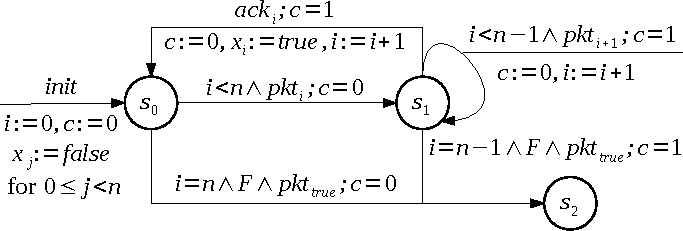
\includegraphics[width=0.45\textwidth]{./figures/sat_sm.pdf}
  \caption{\textbf{Checker State Machine for SAT Problem.}}
  \label{fig:sat}
  \vspace*{-8mm}
\end{wrapfigure}



The protocol checker state machine $S$ is shown in Fig.~\ref{fig:sat}.
%
Initially, all $x_i$ is set to \texttt{false}.
%
At state $s_0$, the DUT shall transmit $pkt_i$ within a unit time, transit to
$s_1$ and reset the clock along the transition.
At state $s_1$, either the DUT receives the $ack_i$ packet and
set $x_i$ to be \texttt{true} ($s_1 \rightarrow s_0$), or the DUT continues to
transmit the next packet $pkt_{i+1}$.
%
After $n$ rounds, the state machine is $s_0$ or $s_1$ depending on whether
$ack_{n-1}$ is received by the DUT.
%
In either case, the DUT shall evaluate $F$ and transmit $pkt_{true}$ if $F$ is
\texttt{true}.  

Consider a sniffer trace $Tr_1=\{(0, pkt_0), (2, pkt_1),\\ (4,
pkt_2),\ldots, (2(n-1), pkt_{n-1}), (2n, pkt_{true})\}$.
%
That is, the sniffer only captures all $pkt_i$ plus the final $pkt_{true}$, but none of
$ack_i$.
%
It is easy to see that $F$ is satisfiable if $S_1^+$ accepts
$Tr_1$.
%
In particular, a successful run of $S_1^+$ on $Tr_1$ would have to
guess, for each $pkt_i$, whether the Type-1 empty transitions should be used
to infer the missing $ack_i$ packet, such that $F$ is \textit{true} at the
end.
%
Note that for $Tr_1$, no Type-2 self transitions can be used since all
packets in $Tr_1$ are sent from the DUT.
%
Therefore, the SAT problem of $F$ can be reduced to the VALIDATION-1 problem
of $S^+_1$ on sniffer trace $Tr_1$.

\sloppy{%
  On the other hand, consider another sniffer trace $Tr_2 =\{(0, pkt_0), (1,
    ack_0), (2, pkt_1), (3, ack_1),\ldots, (2n-2, pkt_{n-1}), (2n-1, ack_{n-1}), (2n,
  pkt_{true}\}$. That is, the sniffer captures all $n$ pair of $pkt_i$ and $ack_i$
  packets and the final $pkt_{true}$ packet.  Similar to $Tr_1$, $F$ is
  satisfiable if $S^+_2$ accepts $Tr_2$. A successful transition sequence of
  $S^+_2$ on $Tr_2$ must decide for each $ack_i$ packet, whether Type-2 self
  transitions should be used, so that $F$ can be evaluated as true at the end.
  Therefore, the SAT problem of $F$ can also be reduced to the VALIDATION-2
  problem of $S^+_2$ on sniffer trace $Tr_2$.
}

Since SAT is known to be NP-complete, both the VALIDATION-1 and the
VALIDATION-2 problem are also NP-complete.

\section{Detail of ARF Algorithm}
Automatic Rate Fallback (ARF)~\cite{kamerman1997wavelan} is the first rate
control algorithm in literature. In ARF, the sender increases the bit rate after
$Th_1$ number of consecutive successes or $Th_2$ number of packets with at most
one retransmission. The sender decreases bit rate after two consecutive packet
failures or if the first packet sent after rate increase (commonly referred as
\textit{probing} packet) fails.

\sloppy{%
  Figure~\ref{fig:arf_sm} shows the state machine $S$ for the packet trace
  collected at sender (DUT), where $DATA_i^r$ denotes a data packet
  with sequence number $i$ and bit rate $r$, $DATA_i^{r\prime}$ is a retransmission packet
  and $Ack$ is the acknowledgment packet. The \texttt{pkg\_succ} function is
  shown in Algorithm~\ref{alg:pkt_succ}.
}

\begin{wrapfigure}{r}{0.45\textwidth}
  \vspace*{-5mm}
  \centering
  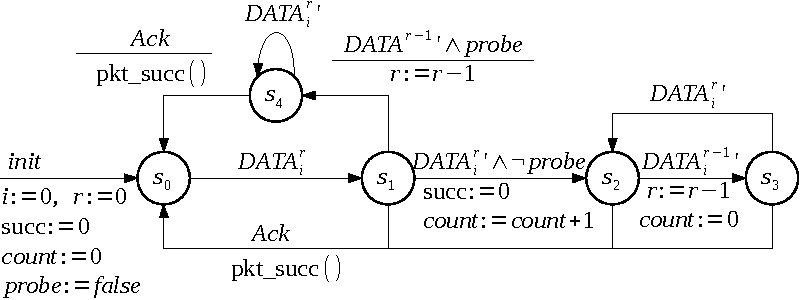
\includegraphics[width=0.45\textwidth]{./figures/arf_sm.pdf}
  \caption{\textbf{Checker State Machine for ARF Rate Control Algorithm.} Timing
  constraints are omitted for succinctness.}
  \label{fig:arf_sm}
  \vspace*{-8mm}
\end{wrapfigure}


The \texttt{succ} variable is used to track the number of consecutive packet
successes. It is increased after each packet success , and is reset to 0 after a
rate increase or upon a packet failure ($s_1\rightarrow s_2$).  Similarly,
\texttt{count} is to track the number of packets with at most one
retransmission, and is increased after packet success, or for the first packet
retransmission ($s_1\rightarrow s_2$). It is reset when there are two
consecutive packet failures ($s_2\rightarrow s_3$). Finally, the \texttt{probe}
flag is set upon rate increases to indicate the probing packet, and is cleared
upon packet success. The variable \texttt{r} is the current bit rate, which is
decreased if the probing packet fails ($s_1\rightarrow s_4$), or every two
consecutive failures ($s_2\rightarrow s_3$). If \texttt{r} is not the highest
rate, it is increased when either of the two thresholds are reached.


\begin{algorithm}[t!]
  \caption{\texttt{pkt\_succ} function}
  \label{alg:pkt_succ}
  \begin{algorithmic}[1]
    \Function{pkt\_succ}{}
    \Let{i}{(i+1)\%N}
    \Let{succ}{succ + 1}
    \Let{count}{count + 1}
    \Let{probe}{false}
    \If{r $< R$ and (succ $\ge Th_1$ or count $\ge Th_2$)}
    \Let{r}{r+1}
    \Let{succ}{0}
    \Let{count}{0}
    \Let{probe}{true}
    \EndIf
    \EndFunction
  \end{algorithmic}
\end{algorithm}

In particular, the bug we found lies in the implementation's \texttt{pkt\_succ}
function in line 6. Instead of checking \texttt{count $\ge$ Th\_2}, the
implementation checks \texttt{count == Th\_2}.

Note that the \texttt{count} variable is incremented twice if a packet succeed
after one retransmission: once in $s_1\rightarrow s_2$, once in the
\texttt{pkt\_succ} function for the retransmission packet. Therefore, if the
value of \texttt{count} is $Th_2-1$ and the next packet succeed after one
retransmission, the value of \texttt{count} will be $Th_2+1$, which would fail
the implementation's test of \texttt{count == Th\_2}.
